\pdfoutput=1  % force pdfLaTeX PDF mode (Overleaf-safe)
% --- self-contained bibliography: writes physweep.bib on compile, so this
% --- single .tex compiles on Overleaf even if uploaded alone -------------
\begin{filecontents}{physweep.bib}
% ===================================================================
% physweep.bib
% Entries located via dated web/arXiv search. Author lists marked with a
% {{double-brace placeholder}} could NOT be confirmed and MUST be filled in
% by the human authors before submission (see README verification checklist).
% Author names are never invented.
% ===================================================================

@inproceedings{kang2025howfar,
  title     = {How Far Is Video Generation from World Model: A Physical Law Perspective},
  author    = {Kang, Bingyi and Yue, Yang and Lu, Rui and Lin, Zhijie and Zhao, Yang and Wang, Kaixin and Huang, Gao and Feng, Jiashi},
  booktitle = {International Conference on Machine Learning (ICML)},
  year      = {2025}
}

@article{motamed2025physicsiq,
  title   = {Do Generative Video Models Understand Physical Principles?},
  author  = {Motamed, Saman and Culp, Laura and Swersky, Kevin and Jaini, Priyank and Geirhos, Robert},
  journal = {arXiv preprint arXiv:2501.09038},
  year    = {2025}
}

@article{bansal2024videophy,
  title   = {{VideoPhy}: Evaluating Physical Commonsense for Video Generation},
  author  = {Bansal, Hritik and Lin, Zongyu and Xie, Tianyi and Zong, Zeshun and Yarom, Michal and Bitton, Yonatan and Jiang, Chenfanfu and Sun, Yizhou and Chang, Kai-Wei and Grover, Aditya},
  journal = {arXiv preprint arXiv:2406.03520},
  year    = {2024}
}

@inproceedings{bansal2025videophy2,
  title     = {{VideoPhy-2}: A Challenging Action-Centric Physical Commonsense Evaluation in Video Generation},
  author    = {Bansal, Hritik and Peng, Clark and Bitton, Yonatan and Goldenberg, Roni and Grover, Aditya and Chang, Kai-Wei},
  booktitle = {International Conference on Learning Representations (ICLR)},
  year      = {2026}
}

@article{zhang2025morpheus,
  title   = {{Morpheus}: Benchmarking Physical Reasoning of Video Generative Models with Real Physical Experiments},
  author  = {{Morpheus Benchmark Authors}},
  journal = {arXiv preprint arXiv:2504.02918},
  year    = {2025}
}

@article{meng2024phygenbench,
  title   = {Towards World Simulator: Crafting Physical Commonsense-Based Benchmark for Video Generation},
  author  = {Meng, Fanqing and Liao, Jiaqi and Tan, Xinyu and Shao, Wenqi and Lu, Quanfeng and Zhang, Kaipeng and Cheng, Yu and Li, Dianqi and Qiao, Yu and Luo, Ping},
  journal = {arXiv preprint arXiv:2410.05363},
  year    = {2024}
}

@article{phyworldbench2025,
  title   = {{PhyWorldBench}: A Comprehensive Evaluation of Physical Realism in Text-to-Video Models},
  author  = {{PhyWorldBench Authors}},
  journal = {arXiv preprint arXiv:2507.13428},
  year    = {2025}
}

@article{inferring2025dynamic,
  title   = {Inferring Dynamic Physical Properties from Video Foundation Models},
  author  = {{Authors of arXiv:2510.02311}},
  journal = {arXiv preprint arXiv:2510.02311},
  year    = {2025}
}

@article{invisiblehand2026,
  title   = {The Invisible Hand of Physics: When Video Diffusion Models Know More Than They Show},
  author  = {{Authors of arXiv:2606.05328}},
  journal = {arXiv preprint arXiv:2606.05328},
  year    = {2026}
}

@article{videorepa2025,
  title   = {{VideoREPA}: Learning Physics for Video Generation through Relational Alignment with Foundation Models},
  author  = {{Authors of arXiv:2505.23656}},
  journal = {arXiv preprint arXiv:2505.23656},
  year    = {2025}
}

@article{travl2025,
  title   = {{TRAVL}: A Recipe for Making Video-Language Models Better Judges of Physics Implausibility},
  author  = {{Authors of arXiv:2510.07550}},
  journal = {arXiv preprint arXiv:2510.07550},
  year    = {2025}
}

@article{vlmcannotreason2026,
  title   = {Vision Language Models Cannot Reason About Physical Transformation},
  author  = {{Authors of arXiv:2603.07109}},
  journal = {arXiv preprint arXiv:2603.07109},
  year    = {2026}
}

@article{vlipp2025,
  title   = {{VLIPP}: Towards Physically Plausible Video Generation with Vision and Language Informed Physical Prior},
  author  = {{Authors of arXiv:2503.23368}},
  journal = {arXiv preprint arXiv:2503.23368},
  year    = {2025}
}

@article{brooks2024sora,
  title   = {Video Generation Models as World Simulators},
  author  = {Brooks, Tim and Peebles, Bill and Holmes, Connor and DePue, Will and Guo, Yufei and Jing, Li and Schnurr, David and Taylor, Joe and Luhman, Troy and Luhman, Eric and Ng, Clarence and Wang, Ricky and Ramesh, Aditya},
  journal = {OpenAI Technical Report},
  year    = {2024}
}

@article{agarwal2025cosmos,
  title   = {Cosmos World Foundation Model Platform for Physical AI},
  author  = {Agarwal, Niket and Ali, Arslan and Bala, Maciej and Balaji, Yogesh and Barker, Erik and Cai, Tiffany and others},
  journal = {arXiv preprint arXiv:2501.03575},
  year    = {2025}
}

@article{blattmann2023svd,
  title   = {Stable Video Diffusion: Scaling Latent Video Diffusion Models to Large Datasets},
  author  = {Blattmann, Andreas and Dockhorn, Tim and Kulal, Sumith and Mendelevitch, Daniel and Kilian, Maciej and Lorenz, Dominik and Levi, Yam and English, Zion and Voleti, Vikram and Letts, Adam and others},
  journal = {arXiv preprint arXiv:2311.15127},
  year    = {2023}
}

@article{yang2024cogvideox,
  title   = {{CogVideoX}: Text-to-Video Diffusion Models with an Expert Transformer},
  author  = {Yang, Zhuoyi and Teng, Jiayan and Zheng, Wendi and Ding, Ming and Huang, Shiyu and others},
  journal = {arXiv preprint arXiv:2408.06072},
  year    = {2024}
}

@article{hacohen2024ltxvideo,
  title   = {{LTX-Video}: Realtime Video Latent Diffusion},
  author  = {{LTX-Video / Lightricks Team}},
  journal = {arXiv preprint arXiv:2501.00103},
  year    = {2024}
}

@article{wan2025,
  title   = {{Wan}: Open and Advanced Large-Scale Video Generative Models},
  author  = {{Wan Team}},
  journal = {arXiv preprint arXiv:2503.20314},
  year    = {2025}
}

@article{xing2024dynamicrafter,
  title   = {{DynamiCrafter}: Animating Open-Domain Images with Video Diffusion Priors},
  author  = {Xing, Jinbo and Xia, Menghan and Zhang, Yong and Chen, Haoxin and Yu, Wangbo and Liu, Hanyuan and Wang, Xintao and Wong, Tien-Tsin and Shan, Ying},
  journal = {arXiv preprint arXiv:2310.12190},
  year    = {2024}
}

@article{karaev2023cotracker,
  title   = {{CoTracker}: It Is Better to Track Together},
  author  = {Karaev, Nikita and Rocco, Ignacio and Graham, Benjamin and Neverova, Natalia and Vedaldi, Andrea and Rupprecht, Christian},
  journal = {arXiv preprint arXiv:2307.07635},
  year    = {2023}
}

@article{bear2021physion,
  title   = {{Physion}: Evaluating Physical Prediction from Vision in Humans and Machines},
  author  = {Bear, Daniel M. and Wang, Elias and Mrowca, Damian and Binder, Felix J. and Tung, Hsiao-Yu Fish and Pramod, R. T. and Holdaway, Cameron and Tao, Sirui and Smith, Kevin and Sun, Fan-Yun and others},
  journal = {arXiv preprint arXiv:2106.08261},
  year    = {2021}
}

@inproceedings{bakhtin2019phyre,
  title     = {{PHYRE}: A New Benchmark for Physical Reasoning},
  author    = {Bakhtin, Anton and van der Maaten, Laurens and Johnson, Justin and Gustafson, Laura and Girshick, Ross},
  booktitle = {Advances in Neural Information Processing Systems (NeurIPS)},
  year      = {2019}
}

@article{huang2024vbench,
  title   = {{VBench}: Comprehensive Benchmark Suite for Video Generative Models},
  author  = {Huang, Ziqi and He, Yinan and Yu, Jiashuo and Zhang, Fan and Si, Chenyang and others},
  journal = {arXiv preprint arXiv:2311.17982},
  year    = {2024}
}

@article{unterthiner2018fvd,
  title   = {Towards Accurate Generative Models of Video: A New Metric and Challenges},
  author  = {Unterthiner, Thomas and van Steenkiste, Sjoerd and Kurach, Karol and Marinier, Raphael and Michalski, Marcin and Gelly, Sylvain},
  journal = {arXiv preprint arXiv:1812.01717},
  year    = {2018}
}

@article{bardes2023vjepa,
  title   = {{V-JEPA}: Latent Video Prediction for Visual Representation Learning},
  author  = {Bardes, Adrien and Garrido, Quentin and Ponce, Jean and Chen, Xinlei and Rabbat, Michael and LeCun, Yann and Assran, Mahmoud and Ballas, Nicolas},
  journal = {OpenReview / arXiv},
  year    = {2023}
}

@article{roadmap2025visualworld,
  title   = {Simulating the Visual World with Artificial Intelligence: A Roadmap},
  author  = {{Visual-World Roadmap Authors}},
  journal = {arXiv preprint arXiv:2511.08585},
  year    = {2025}
}

@article{evolution2026videogen,
  title   = {Evolution of Video Generative Foundations},
  author  = {{Authors of arXiv:2604.06339}},
  journal = {arXiv preprint arXiv:2604.06339},
  year    = {2026}
}

@article{vbench2_2025,
  title   = {{VBench-2.0}: Advancing Video Generation Benchmark Suite for Intrinsic Faithfulness},
  author  = {{VBench-2.0 Authors}},
  journal = {arXiv preprint arXiv:2503.21755},
  year    = {2025}
}

@article{physchoreo2025,
  title   = {{PhysChoreo}: Physics-Controllable Video Generation with Part-Aware Semantic Grounding},
  author  = {{PhysChoreo Authors}},
  journal = {arXiv preprint arXiv:2511.20562},
  year    = {2025}
}

@article{phantom2026,
  title   = {{Phantom}: Physics-Infused Video Generation via Joint Modeling of Visual and Latent Physical Dynamics},
  author  = {{Authors of arXiv:2604.08503}},
  journal = {arXiv preprint arXiv:2604.08503},
  year    = {2026}
}

@article{physvideo2026,
  title   = {{PhysVideo}: Physically Plausible Video Generation with Cross-View Geometry Guidance},
  author  = {Wang, Cong and Zhu, Hanxin and Tang, Xiao and Luo, Jiayi and Jin, Xin and Chen, Long and Wang, Fei-Yue and Chen, Zhibo},
  journal = {arXiv preprint arXiv:2603.18639},
  year    = {2026}
}

@article{motionforcing2026,
  title   = {Motion Forcing: A Decoupled Framework for Robust Video Generation in Motion Dynamics},
  author  = {Xu, Tianshuo and Chen, Zhifei and Wu, Leyi and Lu, Hao and Chen, Ying-cong},
  journal = {arXiv preprint arXiv:2603.10408},
  year    = {2026}
}

@article{diffmemorize2025,
  title   = {How Diffusion Models Memorize},
  author  = {{Authors of arXiv:2509.25705}},
  journal = {arXiv preprint arXiv:2509.25705},
  year    = {2025}
}

@article{lapg2026,
  title   = {Least-Action-Guided Diffusion for Physical Extrapolation},
  author  = {Yang, Zhongxin and Bin, Yuanwei and Yang, Xiang I. A. and Chen, Shiyi},
  journal = {arXiv preprint arXiv:2606.11277},
  year    = {2026}
}

@article{phyground2026,
  title   = {{PhyGround}: Benchmarking Physical Reasoning in Generative World Models},
  author  = {{Authors of arXiv:2605.10806}},
  journal = {arXiv preprint arXiv:2605.10806},
  year    = {2026}
}

@article{phyco2026,
  title   = {{PhyCo}: Learning Controllable Physical Priors for Generative Motion},
  author  = {{Authors of arXiv:2604.28169}},
  journal = {arXiv preprint arXiv:2604.28169},
  year    = {2026}
}

@article{likephys2025,
  title   = {{LikePhys}: Evaluating Intuitive Physics Understanding in Video Diffusion Models via Likelihood Preference},
  author  = {{Authors of arXiv:2510.11512}},
  journal = {arXiv preprint arXiv:2510.11512},
  year    = {2025}
}

@article{t2vphysbench2025,
  title   = {{T2VPhysBench}: A First-Principles Benchmark for Physical Consistency in Text-to-Video Generation},
  author  = {{Authors of arXiv:2505.00337}},
  journal = {arXiv preprint arXiv:2505.00337},
  year    = {2025}
}
\end{filecontents}
\documentclass[10pt]{article}

% ============================================================================
% physweep_main.tex  --  DRAFT (complete pending experiments)
%
% TEMPLATE NOTE FOR THE HUMAN AUTHORS:
%   This file uses a self-contained, ICLR-like single-column preamble so it
%   compiles cleanly anywhere (pdflatex -> bibtex -> pdflatex -> pdflatex)
%   WITHOUT depending on a venue style file that does not exist yet for
%   ICLR 2027. Before submission, replace the geometry/title block below with
%   the OFFICIAL iclr2027_conference.sty (\usepackage{iclr2027_conference})
%   once it is released; the section content maps over unchanged.
% ============================================================================

\usepackage[letterpaper,margin=1in]{geometry}
\usepackage[utf8]{inputenc}
\usepackage[T1]{fontenc}
\usepackage{mathptmx}  % Times (Overleaf-safe; replaces obsolete times.sty)
\usepackage{amsmath,amssymb,amsthm}
\usepackage{graphicx}
\usepackage{booktabs}
\usepackage{array}
\usepackage{caption}
\usepackage{xcolor}
\usepackage{tikz}
\usetikzlibrary{arrows.meta,positioning,calc,backgrounds,fit,patterns}
\usepackage{algorithm}
\usepackage{algpseudocode}
\usepackage[round]{natbib}
\usepackage{hyperref}
\hypersetup{colorlinks=true,linkcolor=blue,citecolor=blue,urlcolor=blue}
\usepackage{enumitem}
\usepackage{pifont}
\newcommand{\cmark}{\textcolor{green!55!black}{\ding{51}}}
\newcommand{\xmark}{\textcolor{red!70!black}{\ding{55}}}

\emergencystretch=3em

% --- Robustness against a stale .aux from a previous compile that used the
% --- lineno package (e.g. an ICLR submission template): absorb its commands
% --- harmlessly so a leftover output.aux cannot break this build. If lineno
% --- is ever loaded, these providecommands defer to its real definitions.
\makeatletter
\providecommand{\@LN@col}[1]{}
\providecommand{\@LN}[2]{}
\makeatother

\newtheorem{proposition}{Proposition}
\newtheorem{definition}{Definition}
\newtheorem{remark}{Remark}
\newtheorem{assumption}{Assumption}

% colors for in-text tags
\newcommand{\torun}[1]{\textcolor{red!70!black}{\textbf{>>> TO RUN:} #1}}
\newcommand{\resph}[1]{\textcolor{blue!60!black}{[RESULT PLACEHOLDER: #1]}}
\newcommand{\PRE}{\ensuremath{\mathrm{PRE}}}
\newcommand{\PRI}{\ensuremath{\mathrm{PRI}}}
\newcommand{\CBI}{\ensuremath{\mathrm{CBI}}}
\newcommand{\EG}{\ensuremath{\mathrm{EG}}}
\newcommand{\thetah}{\ensuremath{\hat{\theta}}}

\title{\textbf{Does the Video Follow the Physics You Asked For?\\
A Label-Free Black-Box Test of Parameter Faithfulness\\
and Extrapolation in Pretrained Video Generators}}

\author{Anonymous Authors\\ Under double-blind review at ICLR 2027}
\date{}

\begin{document}
\maketitle

\begin{abstract}
Pretrained image-to-video (I2V) generators are increasingly described as
implicit ``world models'' that have absorbed physical dynamics from data.
Most evidence for this claim comes from \emph{plausibility} judgments: human
raters or vision-language-model (VLM) auto-raters score whether a clip
``looks physical.'' Plausibility is necessary but not sufficient. A clip can
look perfectly natural while encoding the \emph{wrong} value of the governing
physical parameter. We ask a sharper, falsifiable question: when an I2V model
is conditioned on initial frames that imply a specific physical parameter
(for example a gravitational acceleration, a pendulum frequency, or a
coefficient of restitution), does the generated continuation \emph{realize
that parameter}, and does the relationship hold when the conditioned value is
pushed outside the everyday range? We introduce \textsc{PhysWeep}, a
label-free, automatically verifiable diagnostic that treats a frozen,
off-the-shelf generator as a black-box function from a conditioned control
parameter $\theta$ to a trajectory, recovers the realized parameter
$\thetah$ from the generated pixels by tracking and physics fitting, and
reports a \emph{Parameter Recovery Error} (\PRE), an
\emph{Extrapolation Gap} (\EG) between in-range and out-of-range conditioning,
and two competing failure-form indices, a \emph{Prior-Reversion Index} (\PRI)
for collapse to a single default and a \emph{Case-Based Index} (\CBI) for
mimicry of the nearest seen value. A model-selection rule lets the data decide
which mechanism, if either, the recent literature's two accounts predict.
Because the conditioning is rendered from a deterministic simulator with known
$\theta$, no human annotation is required and every score is exactly checkable.
We further use the same test to audit models that explicitly claim physics
controllability. Our central hypothesis, to be confirmed by the experiments
specified here, is that current open I2V models are faithful in-range but fail
out-of-range in a characterizable way, and that plausibility raters (human,
VLM, and \textsc{VBench-2.0}-style) fail to flag this. We provide the diagnostic
protocol, the parameterized system suite, and the analysis code as a reusable
artifact. \textbf{Quantitative claims in this draft are placeholders until the
specified runs complete.}
\end{abstract}

% ---------------------------------------------------------------------------
\section{Introduction}
% ---------------------------------------------------------------------------

The rapid progress of video generation has revived an old hope: that a model
trained only to predict pixels will, as a by-product, learn the laws that
govern how the world moves \citep{brooks2024sora,agarwal2025cosmos}. If true,
such generators could serve as cheap, general simulators for science and
robotics. The community has accordingly invested heavily in measuring
\emph{physical plausibility} of generated video, through benchmarks that ask
human raters or VLM auto-raters whether motion ``looks right''
\citep{bansal2024videophy,bansal2025videophy2,meng2024phygenbench,motamed2025physicsiq,zhang2025morpheus,phyworldbench2025}.

Plausibility is the wrong target on its own. A generator can produce a clip
that is visually flawless yet encodes a physically \emph{incorrect} value of
the relevant parameter. A ball can fall with a smooth, natural-looking arc
whose implied gravitational acceleration is simply wrong, and no plausibility
rater will object, because the arc is locally consistent. The scientifically
meaningful question is not ``does it look physical'' but ``does it realize the
\emph{specific} physics implied by its conditioning, and does that realization
extend beyond the values the model saw most often during training.'' The
second clause matters because a model that has truly internalized a law should
treat the controlling parameter as a free variable, whereas a model that has
memorized typical motions will fall back on what it has seen whenever it is
pushed away from the common case.

Recent roadmaps single out exactly this gap. Surveys of the field now name
\emph{intrinsic faithfulness} and \emph{controllability} as the defining
frontier for video models as world simulators and note that comprehensive
metrics for it remain underexplored
\citep{roadmap2025visualworld,evolution2026videogen}, and the newest
benchmark suites add ``Physics'' and ``Controllability'' dimensions but score
them with VLM and question-answering proxies rather than exact, swept
measurement \citep{vbench2_2025,t2vphysbench2025,likephys2025}. Such judge-based
scores are hard to reproduce or audit because the judge's weights, versions, and
APIs drift over time \citep{phyground2026}; an exact parameter recovered from
pixels by a fixed estimator does not. The current generation of methods
explicitly \emph{claims} physics controllability and even
beyond-distribution generalization
\citep{physchoreo2025,phantom2026,physvideo2026,phyco2026,motionforcing2026}, and
the very newest work proposes inference-time fixes for physical
\emph{extrapolation} \citep{lapg2026}. None of this work tests whether a
\emph{conditioned} physical parameter is realized in the generated pixels, or
whether that control survives outside the everyday range, and none provides a
fixed, auditable measurement against which such fixes can be checked.

\begin{center}
\fbox{\parbox{0.92\linewidth}{\small
\textbf{Contribution in one statement.} We turn ``physical understanding'' of
a pretrained video generator into a falsifiable measurement: treat the frozen
model as a black-box map from a conditioned control parameter $\theta$ to a
trajectory, recover the realized $\thetah$ from generated pixels with no human
labels, and quantify faithfulness, out-of-range extrapolation, and the
\emph{form} of any failure. Beyond detecting failure, \textsc{PhysWeep}
adjudicates between two mechanisms the recent literature proposes (collapse to
a single global default versus case-based mimicry of the nearest seen value)
and audits the models that explicitly claim physics controllability. The
result is a reusable, model-agnostic diagnostic and a clean separation between
\emph{plausibility} and \emph{parameter faithfulness}.}}
\end{center}

\paragraph{Why prior work does not answer this.}
\citet{kang2025howfar} study generalization (in-distribution, out-of-distribution,
combinatorial) but \emph{train diffusion models from scratch} on a 2D testbed
and report binary success or failure; they characterize the OOD failure as
``case-based'' generalization, where the model mimics the nearest training
example rather than abstracting the law. \citet{invisiblehand2026} corroborate
that scaling fails to extrapolate and probe \emph{internal} states. Neither
recovers a continuous parameter from the generated pixels of a frozen model,
nor adjudicates whether the failure is collapse to one global default or
nearest-value mimicry, nor connects the effect to a controllable knob.
Plausibility benchmarks \citep{motamed2025physicsiq,zhang2025morpheus,bansal2025videophy2,vbench2_2025}
measure adherence on fixed clips, not the response of the model to a
\emph{swept} control parameter. Property-readout methods recover physical
quantities from \emph{input} videos via internal features
\citep{inferring2025dynamic,invisiblehand2026}, which measures what the
encoder represents, not whether the \emph{generated} continuation honors a
requested parameter. \textsc{PhysWeep} fills the gap: a black-box,
generation-side, parameter-swept, label-free test that also names the failure
mechanism and audits models claiming controllability.

\paragraph{Contributions.}
\begin{enumerate}[leftmargin=1.4em,itemsep=2pt,topsep=2pt]
  \item \textbf{A reframing.} We separate \emph{plausibility} from
  \emph{parameter faithfulness} and argue the latter is the operationally
  meaningful sense of ``learning physics from video'' for a generator
  (Section~\ref{sec:problem}).
  \item \textbf{A diagnostic and metrics.} We define \PRE, the Extrapolation
  Gap \EG, a monotonicity score, and two competing failure-form indices, the
  Prior-Reversion Index \PRI\ and the Case-Based Index \CBI, each computable
  label-free with bootstrap confidence intervals, and give an identifiability
  condition under which $\thetah$ is well defined (Section~\ref{sec:metrics}).
  \item \textbf{Adjudicating the failure mechanism.} \PRI\ versus \CBI\ with a
  model-selection criterion lets the data decide between global default
  collapse and case-based nearest-value mimicry, a question the recent
  literature raises but does not test on frozen generators
  (Sections~\ref{sec:problem},~\ref{sec:metrics}).
  \item \textbf{A controllable suite and a controllability audit.}
  \textsc{PhysWeep} ships deterministic, parameterized systems with procedural
  conditioning and ground-truth $\theta$ (Section~\ref{sec:suite}), and applies
  the same test to models that explicitly claim physics controllability or
  improved extrapolation, asking whether the claimed control is faithful and
  whether it survives out of range (Section~\ref{sec:protocol}). Because the
  estimator is fixed and label-free, the measurement is reproducible and
  auditable by construction, unlike evolving VLM-judge scores
  \citep{phyground2026}.
  \item \textbf{A protocol and a falsifiable prediction.} We specify the full
  protocol over open I2V models, with the plausibility-versus-measurement
  contrast as the headline test, and state in advance the results that would
  confirm or refute each hypothesis (Sections~\ref{sec:protocol}--\ref{sec:results}).
\end{enumerate}

% ===================== TEASER (Figure 1) =====================
\begin{center}
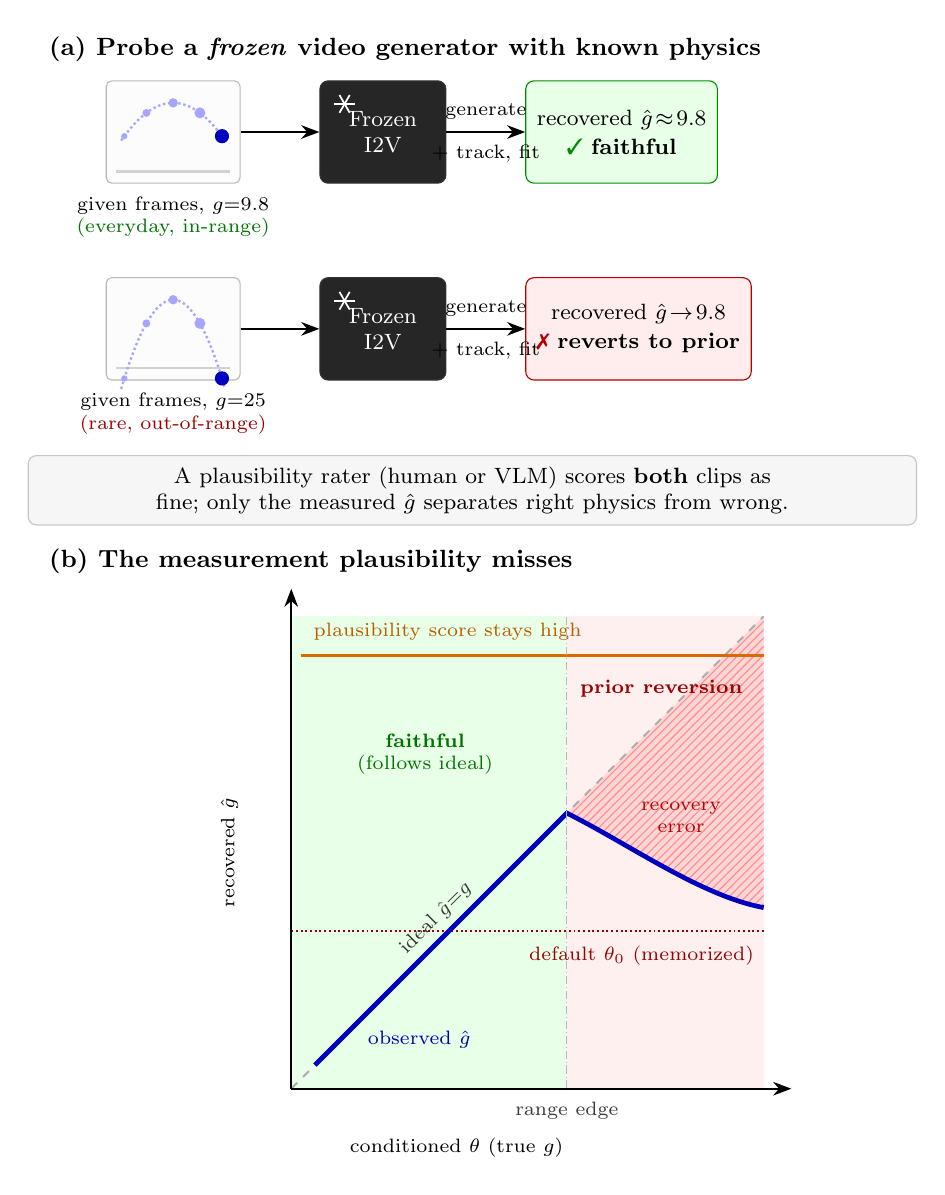
\begin{tikzpicture}[
  font=\footnotesize,
  >={Stealth[length=2.3mm]},
  card/.style={draw=gray!55,fill=gray!2,rounded corners=2pt,minimum width=17mm,minimum height=13mm,inner sep=0pt},
  net/.style={draw=black!80,fill=black!85,text=white,rounded corners=3pt,align=center,inner sep=3pt,minimum height=13mm,minimum width=16mm},
  good/.style={draw=green!55!black,fill=green!9,rounded corners=3pt,align=center,inner sep=4pt,minimum height=13mm,minimum width=24mm},
  bad/.style={draw=red!70!black,fill=red!7,rounded corners=3pt,align=center,inner sep=4pt,minimum height=13mm,minimum width=24mm},
  capt/.style={align=center,font=\scriptsize},
]

% ---- helper: a video-frame card showing a ball on a parabolic arc ----
% #1 node name, #2 curvature k (bigger = steeper/out-of-range)
\newcommand{\arccard}[2]{%
  \begin{scope}[shift={(#1.center)}]
    \draw[gray!35,line width=0.3mm] (-0.72,-0.5) -- (0.72,-0.5); % ground
    \draw[blue!35,densely dotted,line width=0.3mm]
      plot[smooth,domain=-0.66:0.66,samples=20] (\x,{0.42-#2*\x*\x-0.05});
    \foreach \x/\s in {-0.62/0.4,-0.34/0.5,0/0.6,0.34/0.7}
      {\fill[blue!35] (\x,{0.42-#2*\x*\x-0.05}) circle (\s mm);}
    \fill[blue!75!black] (0.62,{0.42-#2*0.62*0.62-0.05}) circle (0.9mm); % current ball
  \end{scope}}
% helper: small white snowflake (frozen marker) at a coordinate
\newcommand{\snow}[1]{\foreach \a in {0,60,120}{%
  \draw[white,line width=0.22mm] ($#1+(\a:1.3mm)$)--($#1+(\a+180:1.3mm)$);}}

% ====================== PANEL (a): the probe (top band) ======================
\node[anchor=west,font=\small\bfseries] at (1.2,13.55)
  {(a) Probe a \emph{frozen} video generator with known physics};

% IN-RANGE row
\node[card] (fin) at (2.9,12.5) {};
\arccard{fin}{1.1}
\node[capt,below=0.4mm of fin] {given frames, $g{=}9.8$\\ \textcolor{green!45!black}{(everyday, in-range)}};
\node[net,right=10mm of fin] (gin) {Frozen\\I2V};
\snow{(gin.north west)+(0.32,-0.3)}
\node[good,right=10mm of gin] (rin) {recovered $\hat g\!\approx\!9.8$\\[1pt]\cmark~\textbf{faithful}};
\draw[->,thick] (fin) -- (gin);
\draw[->,thick] (gin) -- node[above=0.3mm,font=\scriptsize]{generate} node[below=0.3mm,font=\scriptsize]{+ track, fit} (rin);

% OUT-OF-RANGE row
\node[card] (fout) at (2.9,10.0) {};
\arccard{fout}{2.6}
\node[capt,below=0.4mm of fout] {given frames, $g{=}25$\\ \textcolor{red!60!black}{(rare, out-of-range)}};
\node[net,right=10mm of fout] (gout) {Frozen\\I2V};
\snow{(gout.north west)+(0.32,-0.3)}
\node[bad,right=10mm of gout] (rout) {recovered $\hat g\!\to\!9.8$\\[1pt]\xmark~\textbf{reverts to prior}};
\draw[->,thick] (fout) -- (gout);
\draw[->,thick] (gout) -- node[above=0.3mm,font=\scriptsize]{generate} node[below=0.3mm,font=\scriptsize]{+ track, fit} (rout);

% ---- thesis strip between panels ----
\node[draw=gray!45,fill=gray!7,rounded corners=3pt,inner sep=4pt,
      font=\footnotesize,align=center,text width=11cm] at (6.7,7.95)
  {A plausibility rater (human or VLM) scores \textbf{both} clips as fine; only the
   measured $\hat g$ separates right physics from wrong.};

% ====================== PANEL (b): the money plot (bottom) ======================
\node[anchor=west,font=\small\bfseries] at (1.2,7.05)
  {(b) The measurement plausibility misses};

\begin{scope}[shift={(4.4,0.35)}]
  \def\xm{6.0}\def\ym{6.0}\def\xe{3.5}\def\tz{2.0}
  % region shading
  \fill[green!9] (0,0) rectangle (\xe,\ym);
  \fill[red!6]   (\xe,0) rectangle (\xm,\ym);
  % recovery-error wedge (between observed and ideal), filled + hatched
  \fill[red!16]
     (\xe,\xe) .. controls (4.3,3.1) and (5.2,2.45) .. (\xm,2.3) -- (\xm,\xm) -- cycle;
  \fill[pattern=north east lines,pattern color=red!45]
     (\xe,\xe) .. controls (4.3,3.1) and (5.2,2.45) .. (\xm,2.3) -- (\xm,\xm) -- cycle;
  % default theta_0 line
  \draw[densely dotted,red!60!black,line width=0.7pt] (0,\tz) -- (\xm,\tz);
  \node[font=\scriptsize,red!60!black,anchor=north east] at (\xm,\tz-0.06) {default $\theta_0$ (memorized)};
  % ideal identity
  \draw[dashed,gray!65,line width=0.7pt] (0,0) -- (\ym,\ym);
  \node[font=\scriptsize,gray!40!black,rotate=45,anchor=south] at (2.0,2.0) {ideal $\hat g{=}g$};
  % plausibility flat-high line
  \draw[orange!85!black,line width=1pt] (0.12,5.5) -- (\xm,5.5);
  \node[orange!72!black,font=\scriptsize,anchor=south west] at (0.16,5.57) {plausibility score stays high};
  % observed faithfulness curve
  \draw[blue!75!black,line width=1.7pt]
      (0.3,0.3) -- (\xe,\xe) .. controls (4.3,3.1) and (5.2,2.45) .. (\xm,2.3);
  \node[blue!72!black,font=\scriptsize,anchor=west] at (0.85,0.62) {observed $\hat g$};
  % range edge divider
  \draw[densely dashdotted,gray!55] (\xe,0) -- (\xe,\ym);
  % axes
  \draw[->,thick] (0,0) -- (\xm+0.35,0);
  \draw[->,thick] (0,0) -- (0,\ym+0.35);
  \node[font=\scriptsize,anchor=north] at (2.1,-0.5) {conditioned $\theta$ (true $g$)};
  \node[font=\scriptsize,gray!45!black,anchor=north] at (\xe,-0.05) {range edge};
  \node[font=\scriptsize,rotate=90,anchor=south] at (-0.55,\ym/2) {recovered $\hat g$};
  % region annotations
  \node[green!45!black,font=\scriptsize,align=center] at (1.7,4.25) {\textbf{faithful}\\(follows ideal)};
  \node[red!62!black,font=\scriptsize,anchor=south] at (4.7,4.85) {\textbf{prior reversion}};
  \node[red!72!black,font=\scriptsize,align=center] at (4.95,3.45) {recovery\\error};
\end{scope}
\end{tikzpicture}
\captionof{figure}{\textbf{Plausibility is not the same as following the physics
you asked for.} \textbf{(a)} \textsc{PhysWeep} renders conditioning frames from a
deterministic simulator with a known control parameter (here gravity $g$), feeds
them to a \emph{frozen}, off-the-shelf image-to-video generator treated as a
black box, and recovers the realized parameter $\hat g$ from the \emph{generated}
pixels by tracking and physics fitting, with no human labels. For an everyday
value the recovery is faithful; for an out-of-range value the generation falls
back toward a memorized default $\theta_0$, even though a plausibility rater
scores both clips as fine. \textbf{(b)} Sweeping $\theta$ exposes this: $\hat g$
hugs the ideal $\hat g{=}g$ line in-range (green), then bends away out-of-range
(red), opening the hatched recovery-error region while the plausibility score
stays high. The Extrapolation Gap, Prior-Reversion Index, and Case-Based Index
(Section~\ref{sec:metrics}) quantify this region and name the mechanism.
\emph{Curves illustrate the hypothesis under test; they are not measured results.}}
\end{center}

% ---------------------------------------------------------------------------
\section{Related Work}
% ---------------------------------------------------------------------------

\paragraph{Plausibility benchmarks.}
A large family of benchmarks scores whether generated video looks physical:
\textsc{VideoPhy} and \textsc{VideoPhy-2} use human and learned raters of
physical commonsense \citep{bansal2024videophy,bansal2025videophy2};
\textsc{PhyGenBench} and \textsc{PhyWorldBench} expand the taxonomy of laws and
prompts \citep{meng2024phygenbench,phyworldbench2025}; \textsc{Physics-IQ}
covers fluids, optics, solids, magnetism, and thermodynamics on real footage
\citep{motamed2025physicsiq}; \textsc{Morpheus} uses conservation-law metrics on
real experiments \citep{zhang2025morpheus}; \textsc{T2VPhysBench} organizes the
evaluation around first-principles laws \citep{t2vphysbench2025}; and
\textsc{LikePhys} scores intuitive physics by the likelihood a model assigns to
valid versus invalid synthetic pairs \citep{likephys2025}. The newest suite,
\textsc{VBench-2.0}, adds ``Physics'' and ``Controllability'' dimensions but
scores them with VLM and question-answering proxies \citep{vbench2_2025}. All
answer ``does it look right'' or ``does it prefer the valid clip,'' not ``does it
realize a \emph{requested} parameter and extrapolate.''
\textsc{PhysWeep} is complementary and measures the latter.

\paragraph{Reproducibility of physics evaluation.}
\citet{phyground2026} argue that VLM-as-judge benchmarks are difficult to
reproduce or audit because the judge's weights, versions, and APIs evolve, and
that general judges miss subtle violations. \textsc{PhysWeep} sidesteps this: a
parameter recovered from pixels by a fixed, closed-form estimator is
deterministic and re-checkable, independent of any evolving model.

\paragraph{The field's stated frontier.}
Recent roadmaps and surveys argue that video models are progressing from
surface fidelity toward intrinsic faithfulness, controllability, and planning,
and explicitly flag the lack of comprehensive metrics for these properties
\citep{roadmap2025visualworld,evolution2026videogen}. \textsc{PhysWeep}
contributes one such metric for the faithfulness-of-control axis.

\paragraph{Methods that claim controllability or repair extrapolation.}
A wave of 2025--2026 methods inject physical structure to make generation more
controllable or consistent: part-aware editable simulation
\citep{physchoreo2025}, joint visual--physical latent dynamics
\citep{phantom2026}, cross-view geometry guidance \citep{physvideo2026},
ControlNet-based continuous control of friction, restitution, and force with
claimed beyond-simulation generalization \citep{phyco2026}, and decoupled motion
forcing under a quality--consistency--controllability trilemma
\citep{motionforcing2026}. In parallel, inference-time schemes promote physical
\emph{extrapolation} directly \citep{lapg2026}. These are exactly the systems
whose \emph{claimed} control or extrapolation \textsc{PhysWeep} can audit, and it
does so for \emph{frozen, black-box} models, where the gradient or training
access those methods rely on is unavailable (Section~\ref{sec:protocol}).

\paragraph{Generalization and its mechanism.}
\citet{kang2025howfar} find that scaling yields in-distribution success but OOD
failure, with ``case-based'' behavior (mimicking the closest training example,
prioritizing color $>$ size $>$ velocity $>$ shape). The diffusion-memorization
literature links such collapse to overestimation of training modes amplified by
classifier-free guidance \citep{diffmemorize2025}. We turn these observations
into a testable dichotomy on frozen generators (Section~\ref{sec:problem}) and a
guidance-scale ablation (Section~\ref{sec:protocol}).

\paragraph{Reading physics out of video models.}
Recent work recovers physical properties from \emph{input} videos using
internal features \citep{inferring2025dynamic} or probes diffusion-model
states for linearly decodable plausibility \citep{invisiblehand2026}. These
characterize the model's \emph{encoder}. \textsc{PhysWeep} instead measures the
\emph{generation side}: whether the synthesized continuation obeys the
conditioned dynamics, read off the pixels by an external tracker, with no
access to weights or activations.

\paragraph{VLMs as physics judges and physical reasoning datasets.}
VLMs are used to plan plausible generation \citep{vlipp2025} and to judge
implausibility \citep{travl2025}, and recent analyses question whether VLMs
reason about physical transformations at all \citep{vlmcannotreason2026}. We use
a VLM auto-rater only as a \emph{plausibility baseline} to contrast against exact
measurement. Classic vision-physics benchmarks such as \textsc{Physion} and
\textsc{PHYRE} \citep{bear2021physion,bakhtin2019phyre} evaluate prediction or
planning, not the parameter faithfulness of a generative model, and quality
metrics such as FVD and VBench \citep{unterthiner2018fvd,huang2024vbench} are
orthogonal to our question.

% ---------------------------------------------------------------------------
\section{Problem: Plausibility versus Parameter Faithfulness}
\label{sec:problem}
% ---------------------------------------------------------------------------

Let a physical system be governed by a known law $f$ with a scalar control
parameter $\theta \in \Theta \subset \mathbb{R}$ (the framework extends to
vector $\theta$; we use scalar sweeps for clean identifiability). Given an
initial condition $s_0$, the true trajectory is
$\tau_\theta = f(s_0,\theta)$, observed as a short clip of frames.

A generator $G$ is given conditioning frames $c(s_0,\theta)$ rendered from
$\tau_\theta$ and produces a continuation video $v = G(c(s_0,\theta))$. We
\emph{do not} assume access to $G$'s weights, training data, or activations:
$G$ is a black box. An external, model-independent estimator $R$ maps the
generated pixels to a recovered parameter $\thetah = R(v)$ by tracking the
relevant object(s) and fitting $f$.

\begin{definition}[Parameter faithfulness]
$G$ is \emph{$\epsilon$-faithful} on a sweep $S\subseteq\Theta$ if
$\mathbb{E}_{s_0}\,|R(G(c(s_0,\theta)))-\theta| \le \epsilon$ for all
$\theta\in S$.
\end{definition}

Plausibility, by contrast, is a property of $v$ alone: a rater $P(v)\in[0,1]$
scores whether $v$ looks physical, independent of the conditioned $\theta$. The
two come apart precisely when $v$ is locally smooth but encodes the wrong
$\theta$. The empirical core of this paper is to measure how far apart they are
as $\theta$ leaves the common range.

\paragraph{Two hypotheses for out-of-range failure.}
The recent literature offers two distinct accounts of what a generator does
when $\theta$ leaves the common range, and they make different predictions for
$\thetah$ that our sweep can separate. Let $S_\text{in}$ denote the in-range
(common) values.
\begin{itemize}[leftmargin=1.4em,itemsep=2pt,topsep=2pt]
  \item \textbf{H1, global prior reversion.} $\thetah$ is a convex pull toward a
  single default $\theta_0$ (for example a typical Earth gravity), independent
  of where in $S_\text{out}$ the request lies:
  $\thetah \approx \alpha\theta + (1-\alpha)\theta_0$ with a fixed $\theta_0$.
  \item \textbf{H2, case-based mimicry.} $\thetah$ tracks the \emph{nearest
  in-range value} the model has seen \citep{kang2025howfar}, so as $\theta$ grows
  past the range edge $\theta_{\text{edge}}$, $\thetah \approx \theta_{\text{edge}}$
  (it sticks at the boundary of experience rather than collapsing to one center).
\end{itemize}
H1 and H2 coincide only in the special case $\theta_0=\theta_{\text{edge}}$;
in general the curve of $\thetah$ versus $\theta$ in $S_\text{out}$ is flat at
$\theta_0$ under H1 and clamped at $\theta_{\text{edge}}$ under H2. Naming which
holds is itself a finding, and Section~\ref{sec:metrics} gives indices and a
selection rule that let the data decide rather than assuming either.

% ---------------------------------------------------------------------------
\section{Metrics}
\label{sec:metrics}
% ---------------------------------------------------------------------------

Fix a system with sweep grid $\{\theta_i\}_{i=1}^{n}$, partitioned into an
in-range set $S_\text{in}$ (values common in natural video) and an
out-of-range set $S_\text{out}$ (values rare or absent, for example sub-lunar
or super-Jovian gravity). For each $\theta_i$ we draw $m$ initial conditions
and generations and obtain recovered values $\{\thetah_{ij}\}_{j=1}^{m}$.

\paragraph{Parameter Recovery Error (\PRE).}
The normalized recovery error on a set $S$:
\begin{equation}
\PRE(S) \;=\; \frac{1}{|S|}\sum_{\theta_i\in S}
   \frac{1}{m}\sum_{j=1}^{m}
   \frac{\big|\thetah_{ij}-\theta_i\big|}{|\theta_i|+\delta},
\end{equation}
with small $\delta>0$ for numerical stability. Lower is better; $\PRE=0$ is
perfect faithfulness.

\paragraph{Faithfulness slope and monotonicity.}
The least-squares slope $\beta$ of $\thetah$ on $\theta$ over $S_\text{in}$.
A faithful model has $\beta\approx 1$; a model ignoring the conditioning has
$\beta\approx 0$. Because the response may be nonlinear, we also report
Spearman's $\rho$ between $\theta$ and $\thetah$ over the full sweep, which
captures whether the model preserves the \emph{ordering} of requested values
even when the scale is off.

\paragraph{Extrapolation Gap (\EG).}
\begin{equation}
\EG \;=\; \PRE(S_\text{out}) - \PRE(S_\text{in}).
\end{equation}
$\EG\approx 0$ indicates the model extrapolates as well as it interpolates;
$\EG\gg 0$ indicates extrapolation failure localized outside the common range.

\paragraph{Two failure-form indices and a selection rule.}
To adjudicate H1 versus H2 (Section~\ref{sec:problem}) we fit both models to the
out-of-range data and report:
\begin{align}
\text{(H1) shrinkage:}\quad & \thetah = \alpha\,\theta + (1-\alpha)\,\theta_0 + \varepsilon,
   & \PRI &= 1-\hat\alpha, \label{eq:pri}\\
\text{(H2) clamp:}\quad & \thetah = \min(\theta,\theta_{\text{edge}}) + \varepsilon,
   & \CBI &= 1 - \frac{\mathrm{RSS}_{\text{H2}}}{\mathrm{RSS}_{\text{null}}}. \nonumber
\end{align}
$\PRI=0$ means no reversion (the request is followed); $\PRI=1$ means the
output ignores the request and returns the default $\theta_0$. $\CBI$ is the
variance of out-of-range $\thetah$ explained by clamping at the range edge.
We then select between H1 and H2 by held-out fit (leave-one-$\theta$-out $R^2$)
and by the Akaike criterion, reporting which mechanism the data favor per model
and per system, with the possibility that neither fits (a third, model-specific
behavior) reported as such. The default $\theta_0$ and the edge
$\theta_{\text{edge}}$ are reported, not assumed, and $\theta_0$ is additionally
compared to the physically typical value (for gravity, Earth's
$9.81\,\text{m/s}^2$).

\paragraph{Stochasticity.}
Generators are sampled with multiple seeds per condition, yielding a
\emph{distribution} of $\thetah$. We separate two error sources: the bias
$\mathbb{E}[\thetah]-\theta$ (what \PRE\ and the indices above capture) and the
within-condition dispersion $\mathrm{std}(\thetah)$, reported on its own so that
a model that is unbiased-but-noisy is not confused with one that is
biased-but-consistent.

\paragraph{Units and scale.}
We render conditioning ourselves, so the pixel-to-length and frame-to-time
scales are fixed and self-consistent within each clip. To remove any residual
ambiguity from a generator rescaling the scene, all metrics use the
\emph{ratio} $\thetah/\theta$ (equivalently, dimensionless parameters), which is
invariant to a common spatial or temporal rescaling of a clip; an explicit
scale-invariance check is an ablation (Section~\ref{sec:protocol}).

\paragraph{Plausibility-measurement gap.}
For a plausibility rater $P$ (human subset, a VLM auto-rater, and the
\textsc{VBench-2.0} physics/controllability score \citep{vbench2_2025} where
applicable), report mean $P(v)$ alongside \PRE\ on $S_\text{out}$. The headline
quantity is the pair $\big(P(S_\text{out}),\,\PRE(S_\text{out})\big)$: the
hypothesis predicts high $P$ (looks fine) with high \PRE\ (wrong parameter).

\paragraph{Uncertainty.}
All metrics are reported with $95\%$ bootstrap confidence intervals over
$(\theta_i,\text{seed})$ pairs, and the in-range-versus-out-of-range \PRE\
difference is tested with a paired bootstrap (Section~\ref{sec:protocol}).

\subsection{Identifiability of the recovered parameter}

The metrics are only meaningful if $\thetah=R(v)$ is well defined. We state the
condition explicitly rather than burying it.

\begin{assumption}[Trackability and parametric identifiability]
\label{ass:ident}
On the system's clip horizon, (i) the tracked observable (object center,
angle, or contact times) is recoverable from the generated frames up to bounded
noise, and (ii) the map $\theta \mapsto$ (the fitted statistic of $f$) is
injective on $\Theta$.
\end{assumption}

\begin{proposition}[Consistency of $R$ under Assumption~\ref{ass:ident}]
\label{prop:consistency}
If the tracking noise is zero-mean with variance $\sigma^2\to 0$ as frame
resolution and count grow, and $f$ is parameterized so that the fitting
statistic is a continuous injective function of $\theta$, then the
least-squares estimator $\thetah$ converges in probability to the parameter
realized in the trajectory as $\sigma^2\to 0$.
\end{proposition}

\begin{proof}[Proof sketch]
Under injectivity the inverse of the fitting statistic is well defined and, by
continuity, continuous on the compact $\Theta$. The least-squares fit of $f$ is
a continuous functional of the tracked observable; composing with the
continuous inverse and applying the continuous mapping theorem to the
$\sigma^2\to 0$ limit gives convergence in probability. Full statement and the
regularity conditions on $f$ for each system are in Appendix~\ref{app:proof}.
\end{proof}

\begin{remark}[Scope, stated honestly]
Proposition~\ref{prop:consistency} concerns the \emph{estimator} $R$, not the
\emph{generator} $G$. It guarantees that if $G$ produces a trajectory with a
well-defined realized parameter, we can recover it; it makes no claim about
whether $G$'s output is itself governed by a single clean $\theta$. When the
generated motion is not well described by $f$ (for example, the object morphs
or teleports), the fit residual is large; we therefore report a
\textbf{fit-quality gate} ($R^2$ of the physics fit) and treat low-fit
generations as a separate ``non-physical'' category rather than forcing a
$\thetah$. This gate is itself a label-free signal and is reported per system.
\end{remark}

\textbf{This is the only formal claim in the paper, and it is deliberately
about measurement, not about the generator.} Any stronger statement (for
example a guaranteed lower bound on \PRI\ for diffusion models) is left as an
open conjecture; we do not prove it and do not rely on it.

% ---------------------------------------------------------------------------
\section{The \textsc{PhysWeep} Suite}
\label{sec:suite}
% ---------------------------------------------------------------------------

Each system is a deterministic renderer producing (a) conditioning frames, (b)
ground-truth $\theta$, and (c) a single, interpretable sweep axis. Scenes are
intentionally simple and high-contrast so that the external tracker is robust
and Assumption~\ref{ass:ident} is easy to satisfy; this keeps the measurement,
not the perception, in focus.

\begin{center}
\renewcommand{\arraystretch}{1.15}
\resizebox{\columnwidth}{!}{%
\begin{tabular}{@{}llll@{}}
\toprule
\textbf{System} & \textbf{Control $\theta$} & \textbf{Recovered statistic} & \textbf{In / out-of-range example} \\
\midrule
Projectile        & gravity $g$               & parabola curvature $\to g$         & in: $5\text{--}15$; out: $1$ (Moon), $25$ (Jupiter-like) \\
Damped pendulum   & angular freq.\ $\omega$   & zero-crossing period $\to\omega$   & in: typical; out: very short / long period \\
                  & damping $\zeta$           & envelope decay $\to\zeta$          & in: light; out: heavy / near-critical \\
Bouncing ball     & restitution $e$           & bounce-height ratio $\to e$        & in: $0.6\text{--}0.9$; out: $0.2$, $0.99$ \\
Spring--mass      & stiffness $k$             & oscillation period $\to k$         & in: typical; out: very stiff / very soft \\
Inclined slide    & friction $\mu$            & acceleration along slope $\to\mu$  & in: moderate; out: near-frictionless / high \\
\bottomrule
\end{tabular}}
\captionof{table}{The \textsc{PhysWeep} systems. Each has one clean sweep axis
with a closed-form map from a tracked statistic to the parameter, so recovery
is exact and label-free. In/out-of-range splits are defined by what is common
in natural video; exact grids are in Appendix~\ref{app:systems}.}
\end{center}

% ---------------------------------------------------------------------------
\section{Measurement Pipeline}
\label{sec:pipeline}
% ---------------------------------------------------------------------------

\begin{algorithm}[H]
\caption{\textsc{PhysWeep} measurement for one system and one model}
\label{alg:pipeline}
\begin{algorithmic}[1]
\Require frozen generator $G$; sweep grid $\{\theta_i\}$; seeds $\{z_j\}$;
         law $f$; tracker $T$; fit-quality threshold $\rho$
\For{each $\theta_i$ and seed $z_j$}
  \State render conditioning frames $c_{ij}\gets \textsc{Render}(s_0(z_j),\theta_i)$
  \State generate continuation $v_{ij}\gets G(c_{ij})$
  \State track observable $o_{ij}\gets T(v_{ij})$
  \State fit law: $(\thetah_{ij}, R^2_{ij})\gets \textsc{Fit}(f, o_{ij})$
  \If{$R^2_{ij}<\rho$} \State mark $v_{ij}$ \textbf{non-physical} (excluded from \PRE) \EndIf
  \State score plausibility $p_{ij}\gets P(v_{ij})$ \Comment{human subset + VLM rater}
\EndFor
\State compute \PRE, slope $\beta$, \EG, \PRI\ (Eq.~\ref{eq:pri}), with bootstrap CIs
\State \Return metrics, fit-quality rate, plausibility-measurement pairs
\end{algorithmic}
\end{algorithm}

Rendering uses a small deterministic 2D engine (no external assets). Tracking
uses an off-the-shelf point/blob tracker (for example CoTracker
\citep{karaev2023cotracker} or simple color-blob centroiding on the synthetic
scenes, which is robust here). Fitting is closed-form per system
(least-squares parabola, period from zero crossings, envelope decay, bounce
ratios). The pipeline is inference-only and runs on a single 24\,GB GPU.

\paragraph{How $\theta$ is conditioned.}
Image-to-video models accept different inputs, so we specify two conditioning
channels and treat the choice as a controlled axis (ablated in
Section~\ref{sec:protocol}). \textbf{(C1) Frame-implied:} for models that accept
multiple initial frames or a first-and-last frame, we supply rendered frames
whose motion already implies $\theta$ (the parameter is identifiable from the
conditioning itself), and ask the model to continue; faithfulness here means the
continuation keeps the same $\theta$. \textbf{(C2) Text-specified:} for models
that accept one image plus text, we supply a single first frame plus a prompt
that names the regime (for example ``on the Moon'' versus ``on Jupiter'') and
recover $\theta$ from the continuation. C1 isolates dynamics from semantics; C2
tests whether a named control actually moves the realized parameter. Reporting
both prevents attributing a failure of one channel to the model in general.

% ---------------------------------------------------------------------------
\section{Experimental Protocol}
\label{sec:protocol}
% ---------------------------------------------------------------------------

\paragraph{Models (frozen, off-the-shelf, single 24\,GB GPU).}
Open image-to-video generators that run on consumer hardware:
LTX-Video \citep{hacohen2024ltxvideo}, CogVideoX-5B-I2V
\citep{yang2024cogvideox}, and Stable Video Diffusion / DynamiCrafter
\citep{blattmann2023svd,xing2024dynamicrafter}. Optionally a quantized Wan
\citep{wan2025} if it fits. Where weights are available, we additionally probe a
model that \emph{claims} physics controllability
\citep{physchoreo2025,phantom2026,physvideo2026}. \emph{Verify current versions,
licenses, and VRAM at run time and pin them.}

\paragraph{Plausibility baselines.}
A VLM auto-rater prompt for ``is this motion physically plausible'' (report the
exact model and prompt), a small human plausibility subset for calibration, and,
where applicable, the \textsc{VBench-2.0} physics/controllability score
\citep{vbench2_2025}. These are baselines for the contrast, not the main metric.

\paragraph{Statistics.}
$m\ge 5$ seeds per $(\theta_i,\text{model})$; report mean and $95\%$ bootstrap
CIs; test $\PRE(S_\text{out})>\PRE(S_\text{in})$ with a paired bootstrap over
matched initial conditions; report effect sizes, not only $p$-values; for H1
versus H2, report leave-one-$\theta$-out $R^2$ and $\Delta$AIC.

\paragraph{Experiments to run.}
\begin{itemize}[leftmargin=1.4em,itemsep=3pt,topsep=2pt]
  \item \torun{\textbf{E0, pilot (do first).} One system (projectile), one
  model (LTX-Video), 5 in-range and 3 out-of-range $g$ values, 5 seeds each.
  \emph{Decision gate:} if the faithfulness slope $\beta$ on $S_\text{in}$ is
  not detectably positive (CI includes 0), the model ignores the conditioned
  parameter entirely; switch the framing to ``conditioning is not honored.'' Run
  with E6. Supports the central premise; reduces the ``models do not follow
  conditioning at all'' rejection risk.}
  \item \torun{\textbf{E1, faithfulness curve.} Full $g$ sweep, all three
  models, channel C1. Output: $\thetah$-vs-$\theta$ curves, slope $\beta$,
  Spearman $\rho$, $\PRE(S_\text{in})$. Supports Contribution 2.}
  \item \torun{\textbf{E2, extrapolation.} Extend each sweep into $S_\text{out}$;
  compute \EG\ and the paired-bootstrap test. Distinguishes from
  \citet{kang2025howfar} (frozen models, continuous parameter).}
  \item \torun{\textbf{E3, plausibility-measurement gap.} On $S_\text{out}$, pair
  VLM/human/\textsc{VBench-2.0} plausibility with \PRE. Hypothesis: high
  plausibility, high \PRE. Supports Contribution 1; reduces the ``why not just use
  a plausibility benchmark'' risk.}
  \item \torun{\textbf{E4, generality across systems.} Repeat E1--E3 on pendulum,
  bouncing ball, spring, inclined slide. Per-system table. Reduces
  ``single-setting'' risk.}
  \item \torun{\textbf{E5, robustness/ablations (complete set).}
  (a) tracker swap (CoTracker vs blob centroid): metrics must agree, ruling out a
  tracker artifact;
  (b) scale-invariance: rescale object size / clip fps and confirm ratio metrics
  are unchanged;
  (c) object-permanence / fit-quality gate $\rho$ sensitivity and the reported
  non-physical rate;
  (d) conditioning length (frames in C1) and resolution;
  (e) classifier-free guidance scale: test whether higher guidance increases
  \PRI/\CBI, a mechanistic link to memorization \citep{diffmemorize2025};
  (f) prompt phrasing for the C2 channel.
  Reduces ``the effect is a measurement or hyperparameter artifact'' risk.}
  \item \torun{\textbf{E6, negative control.} Feed ground-truth simulator
  continuations (not model outputs) through the identical pipeline; \PRE\ near
  zero, slope near one, fit $R^2$ near one. Validates the measurement.}
  \item \torun{\textbf{E7, failure-mechanism adjudication.} On $S_\text{out}$, fit
  H1 (shrinkage, \PRI) and H2 (clamp, \CBI); select by held-out $R^2$ and
  $\Delta$AIC per model and system; report $\theta_0$ vs $\theta_{\text{edge}}$.
  The contribution the recent literature sets up but does not test on frozen
  models. Supports Contribution 3.}
  \item \torun{\textbf{E8, conditioning-channel ablation.} Run E1--E2 under C1
  (frame-implied) and C2 (text-specified) for models supporting both; compare
  faithfulness and \EG. Separates a dynamics failure from a text-control failure.}
  \item \torun{\textbf{E9, controllability / extrapolation-repair audit.} Apply
  E1--E2 and E7 to a model claiming physics controllability
  \citep{physchoreo2025,phantom2026,physvideo2026,phyco2026} or an
  extrapolation-repair scheme \citep{lapg2026}: does the advertised knob move the
  realized parameter in-range, and does the claimed beyond-range control or
  extrapolation actually hold under exact measurement? Supports Contribution 4;
  high reviewer interest.}
  \item \torun{\textbf{E10, multi-parameter (optional).} Sweep two parameters
  jointly (for example $g$ and $e$) to connect to combinatorial generalization
  \citep{kang2025howfar}; report whether faithfulness on one axis degrades when
  the other is out of range.}
\end{itemize}

% ---------------------------------------------------------------------------
\section{Expected Results and Discussion (placeholders)}
\label{sec:results}
% ---------------------------------------------------------------------------

The tables below are structured for the runs above. \textbf{All numbers are
placeholders until the experiments complete.}

\begin{center}
\renewcommand{\arraystretch}{1.2}
\resizebox{\columnwidth}{!}{%
\begin{tabular}{@{}lcccc@{}}
\toprule
\textbf{Model} & \textbf{slope $\beta$ (in)} & \textbf{$\PRE(S_\text{in})$} & \textbf{$\PRE(S_\text{out})$} & \textbf{\EG} \\
\midrule
LTX-Video        & \resph{$\approx 1$?} & \resph{low?} & \resph{high?} & \resph{$>0$?} \\
CogVideoX-5B-I2V & \resph{} & \resph{} & \resph{} & \resph{} \\
SVD / DynamiCrafter & \resph{} & \resph{} & \resph{} & \resph{} \\
\bottomrule
\end{tabular}}
\captionof{table}{Faithfulness and extrapolation on the projectile system
(E1--E2). The hypothesis predicts $\beta\!\approx\!1$ in-range, low
$\PRE(S_\text{in})$, and $\EG>0$ driven by out-of-range reversion. Values with
$95\%$ bootstrap CIs.}
\end{center}

\begin{center}
\renewcommand{\arraystretch}{1.2}
\resizebox{\columnwidth}{!}{%
\begin{tabular}{@{}lccccc@{}}
\toprule
\textbf{Model} & \textbf{\PRI\ (H1)} & \textbf{\CBI\ (H2)} & \textbf{selected ($\Delta$AIC)} & \textbf{$\theta_0$ vs $\theta_{\text{edge}}$} & \textbf{plausibility $P(S_\text{out})$} \\
\midrule
LTX-Video        & \resph{} & \resph{} & \resph{H1 or H2?} & \resph{} & \resph{high?} \\
CogVideoX-5B-I2V & \resph{} & \resph{} & \resph{} & \resph{} & \resph{} \\
SVD / DynamiCrafter & \resph{} & \resph{} & \resph{} & \resph{} & \resph{} \\
\bottomrule
\end{tabular}}
\captionof{table}{Failure-mechanism adjudication and the plausibility gap
(E3, E7). For each model the data select global prior reversion (H1, high \PRI,
$\theta_0$ near the typical value) or case-based clamping (H2, high \CBI,
$\theta_0\!\approx\!\theta_{\text{edge}}$), or neither. The prediction across all
mechanisms is high plausibility despite large $\PRE(S_\text{out})$.}
\end{center}

\begin{center}
\renewcommand{\arraystretch}{1.2}
\resizebox{\columnwidth}{!}{%
\begin{tabular}{@{}lcccc@{}}
\toprule
\textbf{Controllability-claiming model} & \textbf{slope $\beta$ (in)} & \textbf{$\EG$} & \textbf{selected mechanism} & \textbf{control faithful?} \\
\midrule
Physics-controllable model A & \resph{} & \resph{} & \resph{} & \resph{yes/no?} \\
\bottomrule
\end{tabular}}
\captionof{table}{Controllability audit (E9). Whether a model that
\emph{claims} physics control actually moves the realized parameter in-range
($\beta$) and whether the control survives out of range ($\EG$, mechanism).
A claimed knob with $\beta\!\approx\!1$ in-range but large $\EG$ has
local-only control.}
\end{center}

\paragraph{Reading the outcomes honestly.}
The outcomes are all reportable. (1) \emph{Faithful in-range, fails out-of-range}
with H1 or H2 selected: the headline story, and naming the mechanism is the
contribution. (2) \emph{No conditioning effect} ($\beta\approx 0$): reframe as
``open generators do not honor conditioned dynamics,'' still useful. (3)
\emph{Faithful even out-of-range} ($\EG\approx 0$): a surprising positive result
updating the field toward ``these models have internalized the law,'' reported as
such. (4) \emph{Neither H1 nor H2 fits}: report the observed behavior directly
rather than forcing a label. We commit to reconciling the abstract, title, and
contributions with whichever outcome the data support, and to dropping the
mechanism framing if no mechanism fits.

% ---------------------------------------------------------------------------
\section{Limitations}
% ---------------------------------------------------------------------------
The suite is intentionally synthetic and 2D, which strengthens identifiability
but limits ecological validity; conclusions are about controllable
low-dimensional dynamics, not arbitrary natural scenes. Off-the-shelf I2V
control is imperfect, so the conditioning may not isolate $\theta$ cleanly; the
fit-quality gate and E6 negative control bound this. The default-prior estimate
$\theta_0$ is model-behavioral, not a claim about training data we cannot
observe. Plausibility ``human subset'' is small and for calibration only. None
of these undermine the central measurement, but each bounds its scope.

% ---------------------------------------------------------------------------
\section{Conclusion}
% ---------------------------------------------------------------------------
We reframe ``learning physics from video'' for a generator as a falsifiable,
label-free question of parameter faithfulness and extrapolation, and provide a
black-box diagnostic, metrics with a stated identifiability condition, a
controllable suite, and a protocol whose headline test separates plausibility
from correctness. The artifact is reusable on any image-to-video model. The
empirical claims await the specified runs.

\paragraph{Reproducibility statement.}
All systems are procedurally generated from a seeded deterministic engine;
models are public; trackers and fitting are off-the-shelf or closed-form. The
analysis code (metrics, bootstrap CIs, synthetic smoke test) and the system
generators are released. No human-annotated labels are used. We will fill the
ICLR reproducibility checklist at submission per the current author guide.

\paragraph{Ethics statement.}
The work uses synthetic scenes and public models, with no human-subjects data
beyond a small voluntary plausibility-rating subset (to be collected under the
venue's guidelines). The diagnostic is intended to prevent overclaiming about
video generators as physical simulators, which has safety relevance in robotics
and scientific settings.

\bibliographystyle{plainnat}
\bibliography{physweep}

\appendix
\section{Failure-form index estimation}
\label{app:pri}
\textbf{H1 (shrinkage, \PRI).} Given pairs $(\theta_i,\thetah_{ij})$, fit
$\thetah=\alpha\theta+(1-\alpha)\theta_0$ by least squares with $\theta_0$
either fixed to the physically typical value or estimated jointly; $\PRI=1-\hat\alpha$,
clipped to $[0,1]$. \textbf{H2 (clamp, \CBI).} Fit
$\thetah=\min(\theta,\theta_{\text{edge}})$ with $\theta_{\text{edge}}$ at the
in-range boundary (or estimated); $\CBI=1-\mathrm{RSS}_{\text{H2}}/\mathrm{RSS}_{\text{null}}$.
\textbf{Selection.} Compare H1 and H2 by leave-one-$\theta$-out $R^2$ and by
$\Delta$AIC; if both fits are poor, report the observed behavior without forcing
a label. All confidence intervals use the paired bootstrap over
$(\theta_i,\text{seed})$.

\section{Consistency of the recovery estimator: full statement and proof}
\label{app:proof}
We restate Proposition~\ref{prop:consistency} with explicit regularity
conditions and give the argument in full. The claim concerns only the estimator
$R$, not the generator $G$ (see the Remark in Section~\ref{sec:metrics}).

\textbf{Setup.} Fix a system with law $f$ and scalar parameter
$\theta\in\Theta$, with $\Theta$ a compact interval. A clip of $T$ frames at
resolution scale yields a tracked observable $o\in\mathbb{R}^{d}$ (object
centers, angles, or contact times). Write the population fitting statistic as
$T(\theta)\in\mathbb{R}^{k}$ (for the projectile, the quadratic coefficient of
height versus time; for the pendulum, the mean zero-crossing interval; for the
bouncing ball, the successive height ratio). The estimator forms an empirical
statistic $\hat T$ from $o$ and returns $\thetah=g(\hat T)$, where
$g=T^{-1}$ on the range of $T$.

\textbf{Assumptions.} (A1, trackability) the tracker returns
$\hat o = o^\star + \varepsilon$ with $\mathbb{E}[\varepsilon]=0$ and
$\operatorname{Var}(\varepsilon)=\sigma^2 \Sigma$ for a fixed positive-definite
$\Sigma$, and $\sigma^2\to 0$ as $T$ and the resolution grow; (A2,
identifiability) $T:\Theta\to T(\Theta)$ is injective and continuously
differentiable with $\|T'(\theta)\|\ge c>0$ on $\Theta$; (A3, regularity) the
empirical statistic is a continuous functional $\hat T=\Phi(\hat o)$ with $\Phi$
continuous at $o^\star$ and $\Phi(o^\star)=T(\theta)$.

\begin{proposition}[Consistency, restated]
Under (A1)--(A3), $\thetah=g(\Phi(\hat o)) \xrightarrow{p} \theta$ as
$\sigma^2\to 0$.
\end{proposition}

\begin{proof}
By (A2), $T$ is a continuous injection on the compact set $\Theta$, so its
inverse $g=T^{-1}$ is continuous on $T(\Theta)$ (a continuous bijection from a
compact space to a Hausdorff space is a homeomorphism). By (A1),
$\hat o \xrightarrow{p} o^\star$ since $\operatorname{Var}(\hat o)=\sigma^2\Sigma
\to 0$ and the mean is $o^\star$ (convergence in mean square implies
convergence in probability). By (A3), $\Phi$ is continuous at $o^\star$, so the
continuous mapping theorem gives $\hat T=\Phi(\hat o)\xrightarrow{p}
\Phi(o^\star)=T(\theta)$. Applying the continuous mapping theorem again with the
continuous $g$ yields $\thetah=g(\hat T)\xrightarrow{p} g(T(\theta))=\theta$.
\end{proof}

\textbf{Per-system check of (A2)--(A3).} \emph{Projectile:} $T(\theta)=-\theta/2$
is linear (hence injective, $T'=-1/2$) and $\Phi$ is ordinary least squares on a
quadratic basis, continuous in the data. \emph{Pendulum (small angle):}
$T(\theta)=2\pi/\theta$ on $\theta>0$ is strictly monotone with nonvanishing
derivative on any $\Theta$ bounded away from $0$; zero-crossing interpolation is
continuous where crossings are simple. \emph{Bouncing ball:} the map
$e\mapsto e^2$ from restitution to successive height ratio is injective and
smooth on $(0,1]$. The fit-quality gate ($R^2<\rho$) excludes generations on
which $\Phi$ is ill-posed (object morphs or vanishes), so (A3) is enforced
operationally rather than assumed. \emph{Independent human verification of this
appendix is still required before submission.}

\section{System grids and rendering details}
\label{app:systems}
All scenes are rendered by a seeded deterministic 2D engine at
$256\times256$ over $T{=}24$ frames at $24$ fps, with a single high-contrast
disk (radius $8$ px) on a plain background and a fixed ground line; only the
swept parameter and the seeded initial condition vary within a system. Spatial
and temporal scales are held fixed within a clip, and all metrics use the ratio
$\thetah/\theta$ so the result is invariant to a common rescaling
(Section~\ref{sec:metrics}). The in-range split is centered on values common in
natural video; the out-of-range split probes rare or absent values. Example
grids (final grids are fixed in the released config and reported with results):

\begin{center}
\renewcommand{\arraystretch}{1.15}
\resizebox{\columnwidth}{!}{%
\begin{tabular}{@{}llll@{}}
\toprule
\textbf{System} & \textbf{$\theta$} & \textbf{In-range grid} & \textbf{Out-of-range grid} \\
\midrule
Projectile      & $g$        & $\{5,7,9.8,12,15\}$         & $\{1.6,\,3,\,20,\,25\}$ \\
Damped pendulum & $\omega$   & $\{2,3,4,5\}$ rad/s         & $\{0.5,\,1,\,8,\,12\}$ \\
                & $\zeta$    & $\{0.02,0.05,0.1\}$         & $\{0.3,\,0.6,\,0.9\}$ \\
Bouncing ball   & $e$        & $\{0.6,0.7,0.8,0.9\}$       & $\{0.2,\,0.35,\,0.97\}$ \\
Spring--mass    & $k$        & $\{20,40,60,80\}$ N/m       & $\{5,\,10,\,200,\,400\}$ \\
Inclined slide  & $\mu$      & $\{0.1,0.2,0.3,0.4\}$       & $\{0.01,\,0.7,\,1.0\}$ \\
\bottomrule
\end{tabular}}
\captionof{table}{Example sweep grids per system (illustrative; the released
config fixes the final values). Each row has one swept axis; $m\ge 5$ seeded
initial conditions per grid point.}
\end{center}

\end{document}